\documentclass{standalone}

\usepackage{times}
\usepackage{amsmath}
\usepackage{amssymb}

\usepackage[dvipsnames]{xcolor}
\usepackage{tikz}
\usetikzlibrary{arrows,backgrounds,scopes}

\usepackage{pgfplots}
\pgfplotsset{compat=1.15}
\begin{document}
	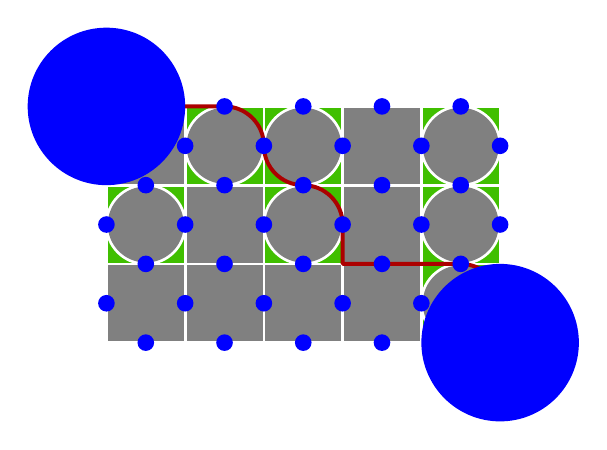
\begin{tikzpicture}[x=1cm,y=1cm]
		%\draw[style=help lines] (0,0) grid (5,3);
		\newlength\gridSize
		\setlength\gridSize{1pt}
		\newcommand{\drawDot}[2]{
			\fill[blue] (#1,#2) circle (3pt);
		}
		\newcommand{\drawO}[2]{
			\fill[green!50!olive] (#1,#2) rectangle (#1+1,#2+1);
			\fill[white] (#1+0.5,#2+0.5) circle (0.5cm+0.5\gridSize);
			\fill[gray] (#1+0.5,#2+0.5) circle (0.5cm-0.5\gridSize);
		}
		\newcommand{\drawX}[2]{
			\fill[gray] (#1,#2) rectangle (#1+1,#2+1);
		}
		\drawX{0}{0}
		\drawO{0}{1}
		\drawX{0}{2}

		\drawX{1}{0}
		\drawX{1}{1}
		\drawO{1}{2}

		\drawX{2}{0}
		\drawO{2}{1}
		\drawO{2}{2}

		\drawX{3}{0}
		\drawX{3}{1}
		\drawX{3}{2}

		\drawO{4}{0}
		\drawO{4}{1}
		\drawO{4}{2}

		\draw[white,line width=\gridSize] (0,0) grid[step=1] (5,3);
		%\draw (0,0) rectangle (5,3);

		\draw[red!50!Maroon!90!black,line cap=round,line width=0.05cm,line join=round] (0,3) -- (1.5,3) arc(90:0:0.5cm) arc(180:270:0.5cm) arc(90:0:0.5cm) -- (3,1) -- (4.5,1) arc(90:0:0.5cm) -- (5,0);
		\fill[red!50!Maroon!90!black] (0,3) circle (2pt);
		\fill[red!50!Maroon!90!black] (5,0) circle (2pt);

		\fill[blue] (5,0) circle (\dotSize);
		\fill[blue] (0,3) circle (\dotSize);

		\foreach \y in {0,...,3}{
			\foreach \x in {0.5,...,4.5}{
				\drawDot{\x}{\y}
			}
		}
		\foreach \y in {0.5,...,2.5}{
			\foreach \x in {0,...,5}{
				\drawDot{\x}{\y}
			}
		}
	\end{tikzpicture}
\end{document}
